\documentclass[10pt]{beamer}

%%%
% PREAMBLE FOR THIS DOC 
%%%
%https://tex.stackexchange.com/questions/68821/is-it-possible-to-create-a-latex-preamble-header
\usepackage{/Users/miw267/Repos/csci246_spring2025/slides/preambles/beamer_preamble_for_CSCI246}


%%% TRY TO RESHOW TOC AT EACH SECTION START (with current section highlighted)
% Reference: https://tex.stackexchange.com/questions/280436/how-to-highlight-a-specific-section-in-beamer-toc
\newcommand\tocforsect[2]{%
  \begingroup
  \edef\safesection{\thesection}
  \setcounter{section}{#1}
  \tableofcontents[#2,currentsection]
  \setcounter{section}{\safesection}
  \endgroup
}


\usepackage[normalem]{ulem} % for strikeout (\sout)

%%%% HERES HOW TO DO IT CORRECTLY
% FIRST IN .STY FILE, DO
%\usetheme[sectionpage=none]{metropolis}
% THEN AT EACH SECTION DO
%\begin{frame}{Outline}
%  \tableofcontents[currentsection]	
%\end{frame}



%\setbeamertemplate{navigation symbols}{}
%\setbeamertemplate{footline}[frame number]{}

%%%
% EVIDENCE CARDS: tinted panel with a coloured accent bar on the left.
% (tcolorbox is already loaded by the preamble.)
%%%
\newtcolorbox{evidence}[1][blue]{%
  enhanced, colback=#1!5, colframe=#1!65,
  boxrule=0pt, leftrule=3pt, arc=0pt, outer arc=0pt,
  left=7pt, right=5pt, top=3pt, bottom=3pt,
  before skip=3pt, after skip=3pt,
  fontupper=\small}
\newcommand{\evsrc}[1]{\par\vspace{1pt}{\tiny\color{black!45}#1}}



%%%
% DOCUMENT
%%%

\begin{document}

%\maketitle

%% Title page frame
%\begin{frame}
%    \titlepage 
%\end{frame}



\title{08/28/2025: Definition}
\author{CSCI 246: Discrete Structures}
\date{Textbook reference: Sec 3, Scheinerman}

\begin{frame}
    \titlepage 
\end{frame}

\begin{frame}
\begin{myyellowbox}[title=Today's Agenda]
\begin{itemize}
	\item Introductory Survey ($\approx$ 5 mins)
	\item Group exercises ($\approx$ 25 mins)
	\item Discussion ($\approx$ 20 minutes)
\end{itemize}


\end{myyellowbox}
\vfill 

\end{frame}




\begin{frame}{Introductory Survey}

\begin{enumerate}
	\item What is your name and major?
	\item What is the most exciting thing about your major?
	\item What do you hope will happen in this class?
	\item What are some concerns you have about this class?
	\item Anything else I should know?
\end{enumerate}
	
\end{frame}



%
%\begin{frame}[standout]
%Q\&A On Previous Group Exercises
%\end{frame}




\begin{frame}{Some virtues of studying definitions}


\begin{evidence}[green]
\textbf{The practical reason.} The rest of the textbook depends heavily on these particular definitions....
%\evsrc{Goodman, \textit{J.\ Labor Economics} 37(4), 2019. \quad Joensen \& Nielsen, \textit{JHR} 44(1), 2009: 20--25\% per advanced course.}
\end{evidence}

	
\end{frame}


\begin{frame}{Some virtues of studying definitions}

\small
\begin{evidence}[orange]
\textbf{Every function signature is a definition.} 
%
\begin{center}
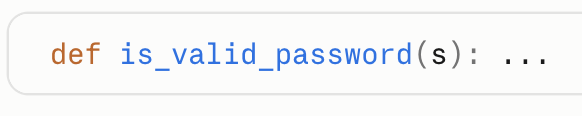
\includegraphics[width=.5\textwidth]{images/password}
\end{center}
%
\end{evidence}

\pause 
\begin{evidence}[blue]
\textbf{Definitions have consequences you can't escape.} Three reasonable-sounding definitions of ``the classifier treats groups fairly'':

\begin{itemize}
\item \textbf{Demographic parity}: the positive rate is the same across groups.
\item \textbf{Equalized odds}: true-positive and false-positive rates match across groups.
\item \textbf{Calibration within groups}: the predictor is well-calibrated separately in each group.
\end{itemize}
\textbf{Theorem} (Kleinberg–Mullainathan–Raghavan 2016; Chouldechova 2017). Except in degenerate cases (equal base rates across groups, or a perfect classifier), these cannot all hold simultaneously. \\
\vspace{.1cm}

Definitions have theorems attached, and you're picking which theorems you get.
%\evsrc{Attridge \& Inglis, \textit{PLoS ONE} 8(7), 2013.}
\end{evidence}
%\begin{evidence}[green]
%\textbf{It pays.} For the marginal student, \textbf{one extra high-school math course $\Rightarrow$ $\sim$10\% higher earnings} via a shift into more cognitively skilled work.
%\evsrc{Goodman, \textit{J.\ Labor Economics} 37(4), 2019. \quad Joensen \& Nielsen, \textit{JHR} 44(1), 2009: 20--25\% per advanced course.}
%\end{evidence}

	
\end{frame}





\begin{frame}{Integers}

\begin{mygreenbox}
\textbf{Definition.} The set of \textit{integers}, denoted $\mathbb{Z}$, is given by
\[\mathbb{Z} \defeq \set{\hdots, -3, -2, -1, 0, 1, 2, 3, \hdots}. \]
That is, the integers are the positive whole numbers, the negative whole numbers, and zero.
\end{mygreenbox}

\end{frame}


\begin{frame}[standout]
Group exercises
\end{frame}

\begin{frame}{Random group assignments}
\footnotesize 
\vfill 
\begin{columns}
\begin{column}{0.33\textwidth}
Ashley, Isabelle: 2 \\ 
Bailey, Tanna: 9 \\ 
Blaisdell, Olyver: 10 \\ 
Brown, Ashton: 12 \\ 
Brown, Jonathan: 9 \\ 
Cardenas, Dominic: 10 \\ 
Cutler, George: 2 \\ 
Fabik, Roland: 9 \\ 
Fellows, Audrey: 1 \\ 
Fitzgerald, Ryan: 6 \\ 
Fuller, Ryan: 8 \\ 
Griffen, Clara: 13 \\ 
Grutsch, Tanner: 11 \\\end{column}
\begin{column}{0.33\textwidth}
Hager, Nathan: 12 \\ 
Horner, Jayden: 3 \\ 
Johnson, Jaret: 7 \\ 
Kintzel, Samantha: 13 \\ 
Lameres, Alexis: 3 \\ 
Lee, Holden: 10 \\ 
Mayala, Reece: 1 \\ 
McLean, Connor: 4 \\ 
Mcbride, Daniel: 7 \\ 
Miller, Maverick: 6 \\ 
Moss, Emily: 1 \\ 
Mousseau, Matthew: 5 \\ 
Neuman, Evan: 3 \\\end{column}
\begin{column}{0.33\textwidth}
Putnam, John: 4 \\ 
Ramos, Vydel: 8 \\ 
Rathbun, Jedidiah: 5 \\ 
Roberts, Matthew: 11 \\ 
Roller, Nathan: 8 \\ 
Ryan, Otis: 6 \\ 
Shevtsov, Timothy: 2 \\ 
Sinclair, Aidan: 7 \\ 
Smith, Charles: 11 \\ 
Stensland, Emma: 12 \\ 
Thiessen, Logan: 4 \\ 
Thompson, Jaiden: 5 \\ 
Vath, Ethan: 13 \\\end{column}
\end{columns}
\vfill
\end{frame}

\begin{frame}{Group exercises}
\begin{enumerate}
\item  Please determine which of the following are true or false; use Definition 3.2 to explain your answers: (a) $3 \mid 100$, (b) $3 \mid 99$, (c) $-3 \mid 3$, (d) $-5 \mid -5$, (e) $-2 \mid -7$, (f) $0 \mid 4$, (g) $4 \mid 0$, (h) $0 \mid 0$.
\item Here is a possible alternative to Definition 3.2: We say that $a$ is \textit{divisible} by $b$ provided $\frac{a}{b}$ is an integer.  Explain why this alternative definition is different from Definition 3.2.  \\
\hspace{0.5cm} Here, \textit{different} means that the definitions specify \textit{different concepts}.  So to answer this question, you should find integers $a$ and $b$ such that $a$ is divisible by $b$ according to one definition, but $a$ is not divisible by $b$ according to the other definition. 
\item None of the following is a prime.  Explain why they fail to satisfy Definition 3.5.  Which of the numbers is composite? (a) 21, (b) 0, (c) $\pi$, (d) $\half$, (e) -2, (f) -1.  
\item Define what it means for an integer to be a \textit{perfect square}.  For example, the integers 0,1,4,9, and 16 are perfect squares.  Your definition should begin: \\
\hspace{0.5cm} An integer $x$ is a \textit{perfect square} provided ...
\end{enumerate}


\end{frame}


\begin{frame}{Solution to group exercise \#1}
%\textbf{Problem.} Please determine which of the following are true or false; use Definition 3.2 to explain your answers.

\begin{mygreenbox}
\textbf{Definition.} Let $a$ and $b$ be integers.  We say $a$ is \textit{divisible} by $b$, written $b \mid a$, provided there is an integer $c$ such that $bc=a$. 	
\end{mygreenbox}
\vspace{-.2cm}
\textbf{Solution.}
\begin{enumerate}[a.]
\item $3 \mid 100$? False. There is no integer $c$ such that $3c=100$.  (Why?  Note that there is exactly one number $c=\frac{100}{3}=33 \frac{1}{3}$ that satisfies the equation, but this $c$ is not an integer.)  
\item $3 \mid 99$? True. There is an integer $c=33$ such that $3c=99$.  
\item $-3 \mid 3$? True. There is an integer $c=-1$ such that $-3c=3$.  
\item $-5 \mid -5$? True. There is an integer $c=1$ such that $-5c=-5$. 
\item $-2 \mid -7$? False. There is no integer $c$ such that $-2c=-7$.   \footnotesize (The number $c=\frac{7}{2}$ uniquely satisfies the equation, but $c$ is not an integer.) \normalsize
\item $0 \mid 4$?  False. There is no integer $c$ such that $0c=4$. (Why?  Note that $0c=0$ for all $c$.)   
\item $4 \mid 0$? True. There is an integer $c=0$ such that $4c=0$.  
\item $0 \mid 0$?  True. There is an integer $c$ such that $0c=0$. In fact, there are \textit{infinitely} many integer-valued solutions!
\end{enumerate}

\end{frame}


\begin{frame}{Solution to group exercise \#2}

\textbf{Problem.} Here is a possible alternative to Definition 3.2: We say that $a$ is \textit{divisible} by $b$ provided $\frac{a}{b}$ is an integer.  Explain why this alternative definition is different from Definition 3.2.  \\
\hspace{0.5cm} Here, \textit{different} means that the definitions specify \textit{different concepts}.  So to answer this question, you should find integers $a$ and $b$ such that $a$ is divisible by $b$ according to one definition, but $a$ is not divisible by $b$ according to the other definition.

 
\vfill 
\textbf{Solution.} Consider $a=b=0$. Then,  $a \mid b$ according to Definition 3.2 (as we discovered in group exercise \#1h). However, $\frac{a}{b}$ is not an integer.
\end{frame}

\begin{frame}{Solution to group exercise \#3 (first part)}
\textbf{Problem.} None of the following numbers is prime. Explain why they fail to satisfy Definition 3.5.
\vfill 

\begin{mygreenbox}
\textbf{Definition.} An integer $p$ is called \textit{prime} provided that $p>1$ and the only positive divisors of $p$ are $p$ and $1$.	
\end{mygreenbox}

\vfill 
\textbf{Solution.}
\begin{enumerate}[a.]
\item 21? This is not prime since $3 \mid 21$, and $3 \not\in \set{1,21}$.  
\item 0?  This is not prime since $0<1$.  
\item $\pi$?  This is not prime since $\pi \not\in \mathbb{Z}$.  
\item $\half$?  This is not prime since $\half \not\in \mathbb{Z}$.  
\item -2?  This is not prime since $-2<1$.  
\item -1?  This is not prime since $-1<1$.  
\end{enumerate}
\vfill \vfill \vfill 
\textbf{Remark.} In the above, I used the shorthand notation $x \not\in A$, which means that $x$ is not a member of the set $A$. 
\end{frame}


\begin{frame}{Solution to group exercise \#3 (second part)}
\textbf{Problem.} None of the following numbers is prime. Which is composite?
\vfill 

\begin{mygreenbox}
\textbf{Definition.} An integer $a$ is called \textit{composite} provided that there is an integer $b$ such that $1<b<a$ and $b \mid a$.	
\end{mygreenbox}

\vfill 
\textbf{Solution.}
\begin{enumerate}[a.]
\item 21?  Composite, since $3 \mid 21$, and $1<3<21$.  
\item 0?  Not composite, since $0<1$.  
\item $\pi$?  Not composite, since $\pi \not\in \mathbb{Z}$.  
\item $\half$?  Not composite, since $\half \not\in \mathbb{Z}$.  
\item -2?  Not composite, since $-2 < 1$.  
\item -1?  Not composite, since $-1 < 1$.  
\end{enumerate}
\vfill 
\textbf{Remark.} Note from the definition that the integer $a$ can be composite only if $a>1$. We use this fact to answer parts b, e, and f.
\end{frame}

\begin{frame}{Solution to group exercise \#4}

\textbf{Problem.} Define what it means for an integer to be a \textit{perfect square}.  For example, the integers 0,1,4,9, and 16 are perfect squares.  

 
\vfill 
\textbf{Solution.} An integer $x$ is a \textit{perfect square} provided there is an integer $y$ such that $x=y^2$.

\end{frame}




\end{document}
